% !TeX root = document.tex
% !TEX program = xelatex
\documentclass[hyperref,a4paper,UTF8]{ctexart}

\usepackage[left=2.50cm, right=2.50cm, top=2.50cm, bottom=2.50cm]{geometry}

\usepackage[unicode=true,colorlinks,urlcolor=black,linkcolor=black,bookmarksnumbered=true]{hyperref}
\usepackage{latexsym,amssymb,amsmath,amsbsy,amsopn,amstext,amsthm,amsxtra,color,bm,calc,ifpdf}
\usepackage{graphicx}
\usepackage{enumerate}
\usepackage{fancyhdr}
\usepackage{listings}
\usepackage{multirow}
\usepackage{makeidx}
\usepackage{xcolor}
\usepackage{fontspec}
\usepackage{subfigure}
\usepackage{hyperref}
\usepackage{pythonhighlight}
\usepackage{float}
\usepackage{subfigure}
\usepackage{natbib} % 用于处理参考文献
\bibliographystyle{abbrv}


\pagestyle{fancy}
\fancyhead[L]{}
\fancyhead[C]{\fangsong 相机标定原理概述}
\fancyhead[R]{}

\renewcommand{\abstractname}{\textbf{\large {摘\quad 要}}} % 更改摘要二字的样式

\title{\textbf{{相机标定原理概述}}}
\author{
\kaishu\normalsize
姓名\ \underline{李康峰} \qquad
学号\ \underline{2201400216} \qquad
院系\ \underline{量新学院} \qquad
班级\ \underline{22工试2班} 
}
\date{\today} % 留空,不显示日期


\begin{document}

\maketitle

\begin{abstract}

本文围绕相机标定这一重要主题展开,着重阐述张正友标定法的原理。介绍了相机标
定的基本概念及其重要性,详细分析张正友标定法的流程,包括棋盘格图像的获取、单应性
矩阵的计算、内参和外参的求解等关键环节,同时探讨该标定法的优势以及应用领域,旨在
让读者深入理解相机标定尤其是张正友标定法在计算机视觉等诸多领域中的关键作用。

\end{abstract}

\

\tableofcontents

\thispagestyle{empty} % 当前页不显示页码
\newpage

\section{引言}

在计算机视觉领域,相机是获取图像信息的关键设备。然而,相机所拍摄的图像往往存
在着畸变等问题,并且相机本身的成像过程涉及到一系列内部和外部参数,这些参数会影响
到后续对图像中物体位置、尺寸等信息的准确判断。相机标定就是通过一定的方法来确定相
机的这些内外部参数的过程,其对于三维重建、目标检测、机器人导航等众多应用场景都有
着至关重要的基础性作用,而张正友标定法以其操作简便、精度较高等优点被广泛应用,下
面将对其原理进行详细概述。

\subsection{相机标定的定义与目标}

相机标定是指确定相机模型中内参、外参以及畸变参数的过程,其目标是将相机捕获的图像坐标系与物理世界的三维坐标系建立精确的映射关系,从而为后续的三维重建、目标定位、物体识别提供数学基础\citep{zhang1998calibration,hartley2004multiple}。

\subsection{相机标定的研究背景}

\begin{itemize}
    \item \textbf{传统方法}:早期方法依赖复杂实验装置(如标定立方体),步骤繁琐且精度受限。
    \item \textbf{现代方法}:基于特征检测的标定方法,尤其是张正友标定法,因其灵活性和高效性被广泛采用。
\end{itemize}

\section{相机成像模型}

理解相机标定的核心在于建立准确的相机成像模型。本节将从数学角度分析相机成像原理。

\subsection{针孔相机模型}

在针孔相机模型中,成像过程是通过光线通过一个点投射到图像平面上来描述的。模型的基本假设是,世界坐标系中的点 $P(X, Y, Z)$ 经过投影映射到图像坐标系中的点 $p(u, v)$。如图 \ref{fig:pinhole} 所示,投影的过程可以通过以下公式表示:

\begin{equation}
    \begin{bmatrix}
        u \\ v \\ 1
    \end{bmatrix}
    =
    K \cdot
    \begin{bmatrix}
        R & t \\
        0 & 1
    \end{bmatrix}
    \cdot
    \begin{bmatrix}
        X \\ Y \\ Z \\ 1
    \end{bmatrix}
\end{equation}

其中,$K$ 为内参矩阵,$R$ 为旋转矩阵,$t$ 为平移向量。该公式通过旋转和平移操作,将三维世界坐标系中的点投影到二维图像坐标系中。

\begin{figure}[h]
    \centering
    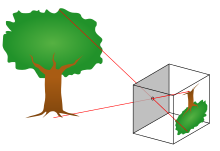
\includegraphics[width=0.45\textwidth]{assets/pinhole_image.png}
    \caption{针孔相机模型示意图:光线从世界坐标系点 $P(X, Y, Z)$ 投射到图像平面上,形成图像坐标系点 $p(u, v)$。}
    \label{fig:pinhole}
\end{figure}

图 \ref{fig:pinhole_geometry} 进一步展示了针孔相机模型中的几何关系。

\begin{figure}[h]
    \centering
    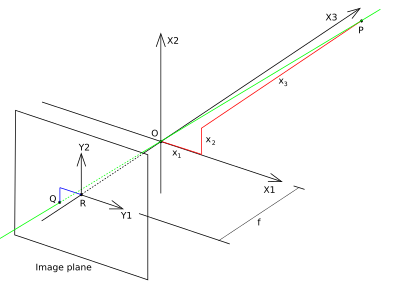
\includegraphics[width=0.45\textwidth]{assets/pinhole_geometry.png}
    \caption{针孔相机模型的几何结构:描述了相机的成像过程以及世界坐标系到图像坐标系的映射关系。}
    \label{fig:pinhole_geometry}
\end{figure}

\subsection{畸变模型}

实际相机存在镜头畸变问题,主要分为以下两种:

\begin{itemize}
    \item \textbf{径向畸变}:由镜头形状导致,公式为 $r' = r(1 + k_1r^2 + k_2r^4 + \dots)$,其中 $r$ 为像素坐标的径向距离,$k_1, k_2, \dots$ 为径向畸变系数。
    \item \textbf{切向畸变}:由镜头装配不对称导致,公式为 $x' = x + [2p_1xy + p_2(r^2 + 2x^2)]$,其中 $p_1, p_2$ 为切向畸变系数,$r$ 为像素的径向距离,$x, y$ 为像素坐标。
\end{itemize}

下面的图像展示了不同类型的畸变效果:

\begin{figure}[h]
    \centering
    \subfigure[桶形畸变]{
        
\includegraphics[width=0.3\textwidth]{assets/100px-Barrel_distortion.svg.png}
        \label{fig:barrel_distortion}
    }
    \subfigure[胡须形畸变]{
        
\includegraphics[width=0.3\textwidth]{assets/100px-Mustache_distortion.svg.png}
        \label{fig:mustache_distortion}
    }
    \subfigure[枕形畸变]{
        
\includegraphics[width=0.3\textwidth]{assets/100px-Pincushion_distortion.svg.png}
        \label{fig:pincushion_distortion}
    }
    \caption{不同类型的镜头畸变效果示意图,包括桶形畸变、胡须形畸变和枕形畸变。}
\end{figure}

\section{张正友标定法原理与步骤}

张正友标定法通过棋盘格图像求解相机参数,其具体流程如下。

\subsection{棋盘格图像的拍摄与预处理}

为了进行相机标定,需要拍摄一系列标准棋盘格图像,这些图像需要在多个角度下进行拍摄,以确保覆盖不同的视角和深度信息。这些图像中需要包含尽可能多的棋盘格角点,以便在标定过程中准确计算相机的内外参数。拍摄时应确保棋盘格的每个角点都清晰可见,并避免模糊或失焦。

在图像的预处理阶段,主要包括以下步骤:

\begin{itemize}
    \item \textbf{图像灰度化处理}:首先将原始彩色图像转换为灰度图像。灰度化有助于减少计算复杂度,同时去除颜色信息,仅保留亮度信息,这对于角点检测至关重要。
    \item \textbf{亚像素级角点检测}:传统的角点检测方法(如Harris角点检测)能检测到较粗略的角点位置,而为了提高检测精度,进一步使用亚像素级角点检测。该方法可以在检测到的角点位置基础上,进一步精确到像素级别甚至亚像素级别,提高后续标定的精度。
\end{itemize}

以下展示了棋盘格图像的预处理过程:图\ref{fig:chessboard_raw}为未检测角点的原始棋盘格图像,而图\ref{fig:chessboard_detected}则展示了经过亚像素级角点检测后的结果。

\begin{figure}[h]
    \centering
    \subfigure[未检测角点的棋盘格图像]{
        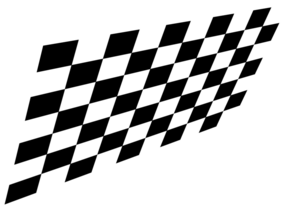
\includegraphics[width=0.45\textwidth]{assets/292px-Perspective_chessboard.png}
        \label{fig:chessboard_raw}
    }
    \subfigure[检测角点的棋盘格图像]{
        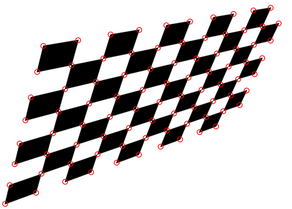
\includegraphics[width=0.45\textwidth]{assets/292px-Harris_corners_detected_on_chessboard.png}
        \label{fig:chessboard_detected}
    }
    \caption{棋盘格图像的拍摄与角点检测过程。左图为原始图像,右图为经过亚像素级角点检测后的图像,显示了图像中检测到的角点位置。}
\end{figure}

\subsection{单应性矩阵的求解}

单应性矩阵(Homography Matrix)描述了一个二维平面到图像平面的映射关系。给定世界坐标系中的棋盘格角点与图像坐标系中的对应点,单应性矩阵 $\mathbf{H}$ 可以通过下式计算:

\begin{equation}
    \mathbf{H} = \mathbf{A}^{-1}\mathbf{B}
\end{equation}

其中,$\mathbf{A}$ 和 $\mathbf{B}$ 分别表示世界坐标系和图像坐标系的相关矩阵。通过解线性方程组,可以求得该矩阵 $\mathbf{H}$,从而实现世界坐标到图像坐标的映射\citep{zhang1998calibration}。

图\ref{fig:homography_transform}展示了二维平面图像在单应性变换下的效果,左侧为原始图像,右侧为经过单应性变换后的图像,变换后的图像能更好地匹配实际的图像平面。

\begin{figure}[h]
    \centering
    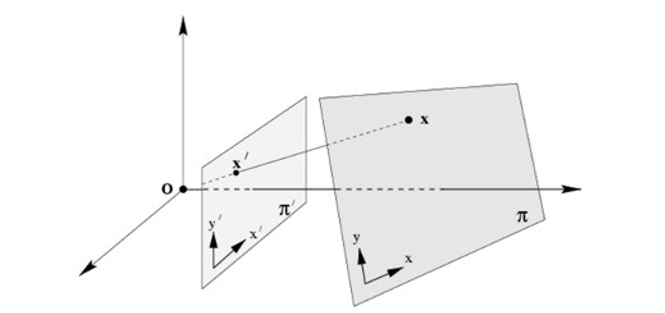
\includegraphics[width=0.8\textwidth]{assets/homography_transform.png}
    \caption{二维平面的单应性变换结果。左图为原始图像,右图为单应性变换后的图像,展示了平面到图像平面的映射效果。}
    \label{fig:homography_transform}
\end{figure}

\subsection{内参、外参的求解}

通过多张图像的单应性矩阵,构建全局优化问题,联合求解内参和外参矩阵。公式如下\citep{tsai1987calibration}:
\begin{equation}
    J = \sum_{i=1}^{N} ||\mathbf{p}_i - \hat{\mathbf{p}}_i||^2
\end{equation}

\subsection{畸变参数的标定}

在相机标定中,畸变参数的精确标定对于提高图像质量至关重要。通过非线性优化方法,如 Levenberg-Marquardt 算法,可以对径向和切向畸变进行优化\citep{weng1992camera}。这种方法通过最小化重投影误差来迭代更新畸变参数,从而有效矫正图像中的畸变。

图\ref{fig:distortion_correction}展示了通过标定优化前后棋盘格图像的畸变效果。左侧为原始畸变图像,右侧为矫正后的图像,显示了径向和切向畸变的校正效果。

\begin{figure}[h]
    \centering
    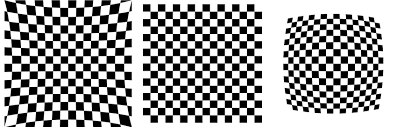
\includegraphics[width=0.8\textwidth]{assets/checkerboard_distort_compare.png}
    \caption{畸变参数优化效果图,展示了棋盘格图像矫正前后的对比。}
    \label{fig:distortion_correction}
\end{figure}

\subsection{重投影误差分析}

重投影误差是衡量相机标定精度的重要指标,其定义为图像中实际角点位置与通过标定计算得到的角点位置之间的差异。重投影误差 $e$ 的计算公式如下:

\begin{equation}
    e = \frac{1}{N}\sum_{i=1}^{N} ||p_i - \hat{p}_i||
\end{equation}

其中,$p_i$ 是实际图像中的角点位置,$\hat{p}_i$ 是通过标定模型计算得到的预测角点位置,$N$ 是角点的总数。重投影误差的大小反映了标定精度的高低。

图\ref{fig:reprojection_error}展示了重投影误差的分布情况,图中显示了标定过程中每个角点的误差值,误差分布的宽度和形态可以为进一步的标定优化提供依据。

\begin{figure}[h]
    \centering
    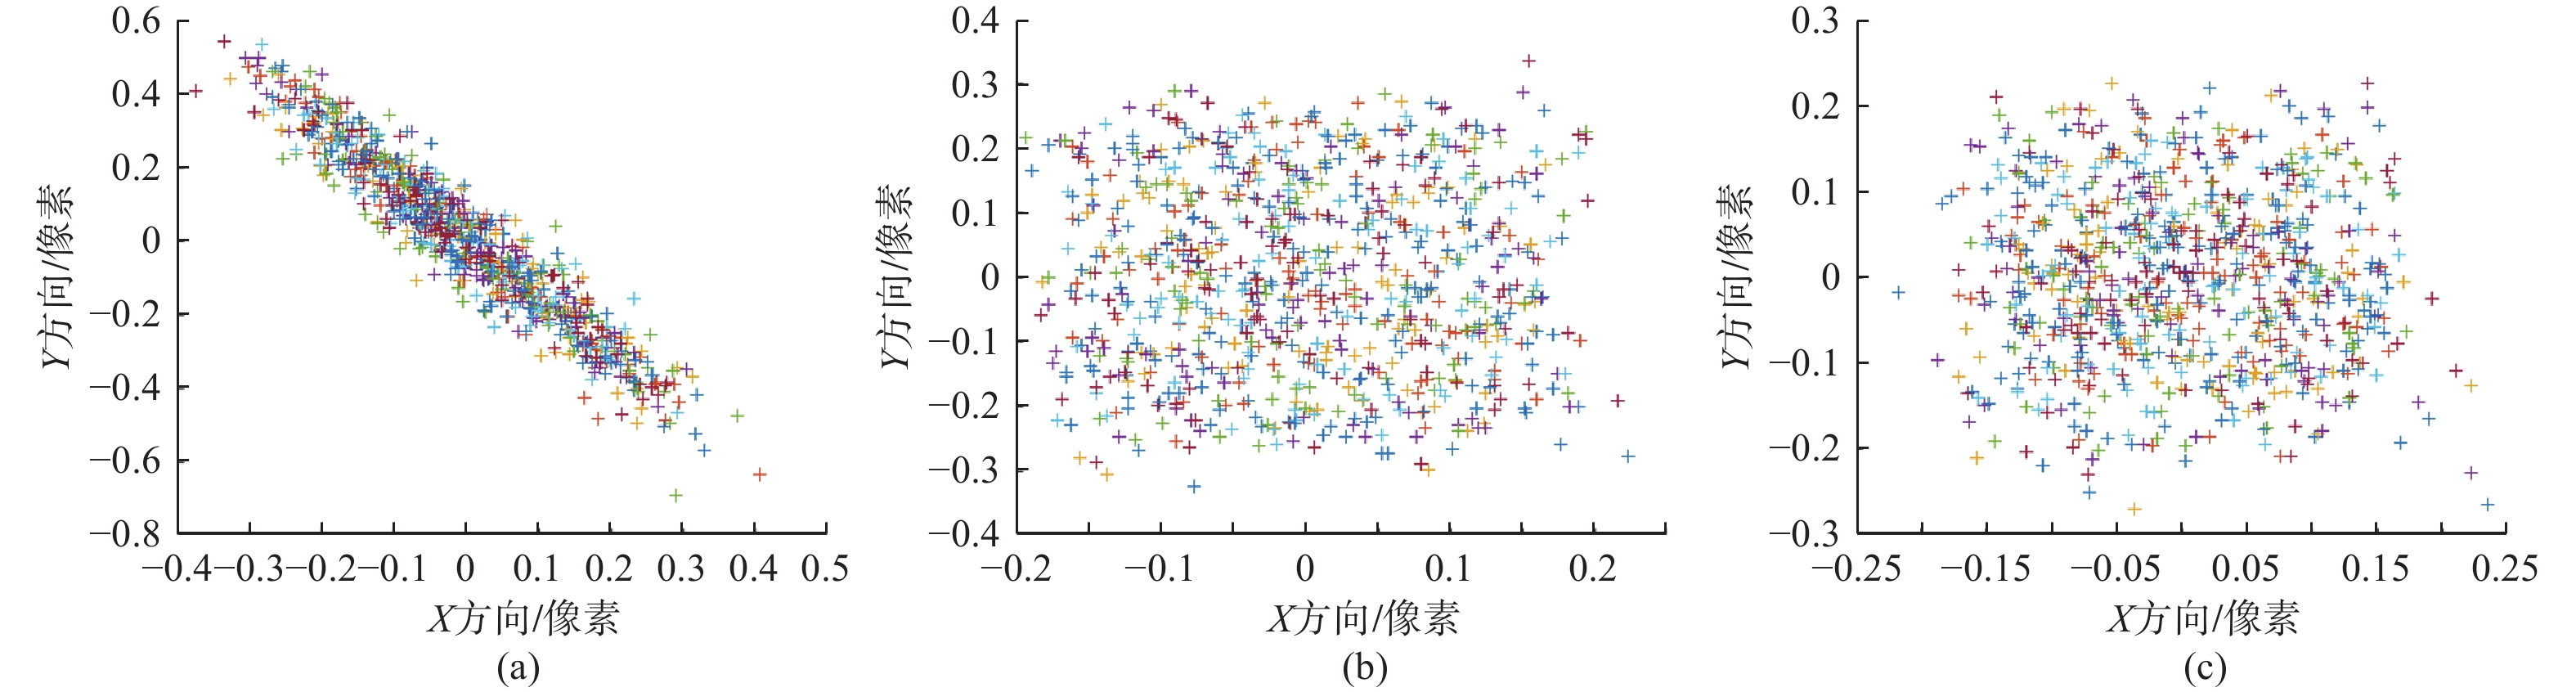
\includegraphics[width=0.8\textwidth]{assets/重投影误差分布.jpg}
    \caption{重投影误差分布图,展示了标定过程中每个角点的误差分布情况。}
    \label{fig:reprojection_error}
\end{figure}

\section{实验与分析}

在实际标定任务中,使用张正友标定法进行相机标定,具体实验步骤和结果如下:

\begin{itemize}
    \item 数据采集:使用了 20 张不同角度拍摄的棋盘格图像,这些图像确保了丰富的角点信息。
    \item 标定结果:标定后得到的内参矩阵和畸变系数如下所示。
\end{itemize}

为了更好地理解标定过程的效果,图\ref{fig:multiple_chessboards} 展示了包含20张合并棋盘格图像的重建效果。这些图像展示了不同视角下的标定过程,经过标定后,重投影误差得到显著降低。

\begin{figure}[h]
    \centering
    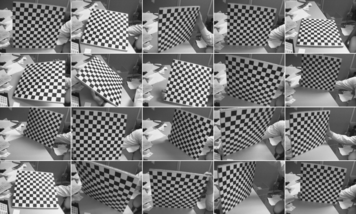
\includegraphics[width=\textwidth]{assets/356px-Multiple_chessboard_views.png}
    \caption{标定过程中的多个棋盘格视角图像,展示了不同视角下的标定效果。}
    \label{fig:multiple_chessboards}
\end{figure}

为了进一步展示标定精度,图\ref{fig:reconstructed_boards_camera} 展示了标定后的重建棋盘格图像,证明了标定过程的成功。

\begin{figure}[H]
    \centering
    \begin{minipage}{0.48\textwidth}
        \centering
        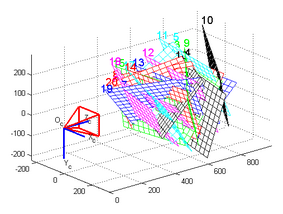
\includegraphics[width=\textwidth]{assets/283px-Reconstructed_boards_camera.png}
        \caption{标定后的重建棋盘格图像(相机视角)。}
        \label{fig:reconstructed_boards_camera}
    \end{minipage}
    \hfill
    \begin{minipage}{0.48\textwidth}
        \centering
        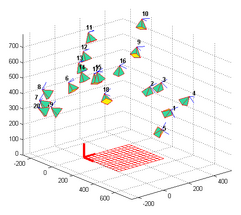
\includegraphics[width=\textwidth]{assets/241px-Reconstructed_boards_world.png}
        \caption{标定后的重建棋盘格图像(世界坐标视角)。}
        \label{fig:reconstructed_boards_world}
    \end{minipage}
\end{figure}

\section{结论与展望}

相机标定技术在三维重建、机器人导航和工业视觉中得到了广泛应用。例如,张正友标定法在机器人手眼系统中用于精确估计相机姿态,从而实现高精度的抓取任务\citep{bouguet2001camera}。

随着深度学习的普及,基于神经网络的无模板标定方法成为研究热点。然而,传统方法(如张正友标定法)仍以其理论稳健性和可解释性在许多工业场景中占据主导地位\citep{ma2003invitation}。

\bibliography{document}  

\end{document}
